\documentclass[10pt]{article}
\usepackage[ngerman]{babel}
\usepackage[utf8]{inputenc}
\usepackage[T1]{fontenc}
\usepackage{amsmath}
\usepackage{amsfonts}
\usepackage{amssymb}
\usepackage[version=4]{mhchem}
\usepackage{stmaryrd}
\usepackage{bbold}
\usepackage{graphicx}
\usepackage[export]{adjustbox}
\graphicspath{ {./images/} }

\title{Hauptprüfung Abiturprüfung 2023 - Leistungsfach }

\author{Alexander Schwarz\\
www.mathe-aufgaben.com}
\date{}


\begin{document}
\maketitle
 Baden-Württemberg

\section*{Aufgabe A 1.1 (15 VP)}
Für jedes $t \in \mathbb{R}_{0}^{+}$ist $G_{t}$ der Graph der Funktion $f_{t}$ mit $f_{t}(x)=\left(1-t x^{2}\right) \cdot e^{-2 x}, x \in \mathbb{R}$.\\
a) Zeigen Sie , dass der Schnittpunkt von $\mathrm{G}_{\mathrm{t}}$ mit der $y$-Achse unabhängig von $t$ ist. (0,5 VP)\\
Entscheiden Sie, welcher der abgebildeten Graphen $\mathrm{G}_{10}$ dargestellt, und begründen Sie Ihre Entscheidung. (1 VP)\\
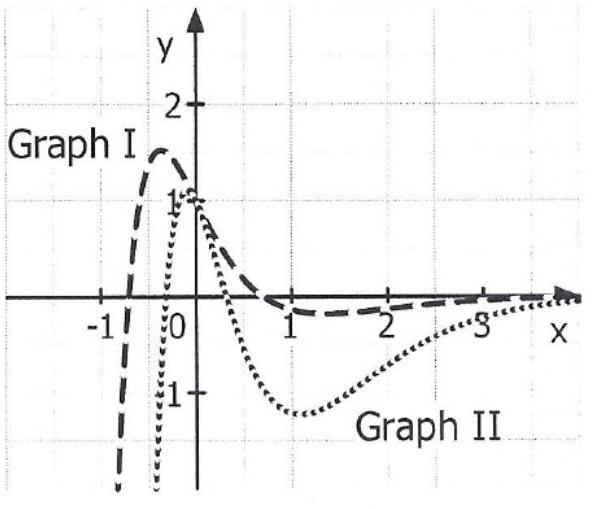
\includegraphics[max width=\textwidth, center]{2025_04_24_90a5eda6f4e325482b12g-2}\\
b) Begründen Sie, dass $f_{0}$ umkehrbar ist.

Ermitteln Sie einen Term der Umkehrfunktion von $f_{0}$ und geben Sie die Definitionsmenge dieser Umkehrfunktion an.\\
c) Betrachtet wird die Tangente an $\mathrm{G}_{0}$ im Punkt $\mathrm{B}\left(0,5 \mid \mathrm{f}_{0}(0,5)\right)$.

Bestimmen Sie die Größe des Schnittwinkels dieser Tangente mit der x-Achse.\\
(1 VP)\\
Diese Tangente begrenzt mit den Koordinatenachsen ein rechtwinkliges Dreieck. Berechnen Sie die Längen der Katheten dieses Dreiecks exakt.\\
(1,5 VP)\\
Bei Rotation dieses Dreiecks um die x- bzw. y-Achse entsteht jeweils ein Körper. Interpretieren Sie in diesem Zusammenhang folgende Ungleichung geometrisch:


\begin{equation*}
\frac{2 \pi}{3 \mathrm{e}}>\frac{4 \pi}{3 \mathrm{e}^{2}} \tag{1,5VP}
\end{equation*}


d) Für einen bestimmten Wert von $t$ besitzt der Graph $G_{t}$ zwei Schnittpunkte mit der x-Achse, die voneinander den Abstand 8 haben.\\
Berechnen Sie diesen Wert von $t$.\\
e) Die Funktion $H$ mit $H(x)=-\left(x^{2}+x+\frac{1}{2}\right) \cdot e^{-2 x}$ ist eine Stammfunktion von $h$ mit $h(x)=f_{t}(x)-f_{t+2}(x)$. Die Graphen $G_{t}$ und $G_{t+2}$ besitzen für $x>0$ keine gemeinsamen Punkte und schließen mit der y-Achse eine nach rechts unbegrenzte Fläche ein. Bestimmen Sie den Inhalt dieser Fläche.\\
f) Für jedes $t>0$ hat der Graph $G_{t}$ zwei Extrempunkte $P_{t}$ und $Q_{t}$. Begründen Sie, dass der Mittelpunkt der Strecke $P_{t} Q_{t}$ auf der Gerade mit der Gleichung $x=\frac{1}{2}$ liegt.

\section*{Aufgabe A 1.2 (5 VP)}
Gegeben ist eine Schar von Funktionen $f_{k}$ mit $k>0$, deren Ableitungsfunktionen $f_{k}^{\prime}$ folgende Gleichung besitzen:

$$
f_{k}^{\prime}(x)=-\frac{1}{k^{2}}(x-k)(x+3 k)
$$

a) Jeder Graph der Schar besitzt einen Wendepunkt. Betrachtet werden die Tangenten in diesen Wendepunkten. Zeigen Sie, dass alle diese Wendetangenten parallel zueinander sind.\\
b) Jeder Graph der Schar hat einen Extrempunkt im ersten Quadranten. Alle diese Extrempunkte liegen auf der ersten Winkelhalbierenden. Bestimmen Sie eine Funktionsgleichung von $f_{k}$.

\section*{Lösungen}
\section*{Aufgabe A 1.1}
a) Zeigen Sie, dass der Schnittpunkt von $\mathrm{G}_{\mathrm{t}}$ mit der y-Achse unabhängig von tist.\\
$f_{t}(0)=(1-0) \cdot e^{0}=1$

Der Schnittpunkt $\mathrm{S}_{\mathrm{y}}(0 \mid 1)$ ist unabhängig von t .\\
Entscheiden Sie, welcher der abgebildeten Graphen $\mathrm{G}_{10}$ dargestellt, und begründen Sie Ihre Entscheidung.

Es gilt $\mathrm{f}_{10}(1)=(1-10) \cdot \mathrm{e}^{-2} \approx-1,22$.\\
Da der Punkt A(1|-1,22) auf dem Graphen $G_{10}$ liegt, muss Graph II der Graph $G_{10}$ sein.\\
b) Begründen Sie, dass $\mathrm{f}_{0}$ umkehrbar ist.

Es gilt $f_{0}(x)=e^{-2 x}$.\\
Die Funktion $f_{0}$ ist streng monoton fallend, da $f_{0}^{\prime}(x)=-2 e^{-2 x}<0$ ist.\\
Daher ist $f_{0}$ umkehrbar.

Ermitteln Sie einen Term der Umkehrfunktion von $\mathrm{f}_{0}$ und geben Sie die\\
Definitionsmenge dieser Umkehrfunktion an.\\
$y=e^{-2 x}$\\
Tausch der Variablen: $x=e^{-2 y}$\\
Auflösen nach $y$ : $-2 y=\ln (x) \Leftrightarrow y=-\frac{1}{2} \ln (x)$\\
Term der Umkehrfunktion: $\overline{\mathrm{f}_{0}}(\mathrm{x})=-\frac{1}{2} \ln (\mathrm{x})$\\
Definitionsmenge: $\left.\mathrm{D}_{\overline{\mathrm{f}}_{0}}=\right] 0 ;+\infty[$\\
c) Bestimmen Sie die Größe des Schnittwinkels dieser Tangente mit der x-Achse.

Steigung der Tangente:\\
Es gilt $f_{0}^{\prime}(x)=-2 e^{-2 x}$.\\
Daraus folgt $f_{0}^{\prime}(0,5)=-2 e^{-1}$\\
Steigungswinkel der Tangente: $\tan (\alpha)=\mathrm{m} \Leftrightarrow \tan (\alpha)=-2 \mathrm{e}^{-1} \Leftrightarrow \alpha \approx-36,3^{\circ}$\\
Der Steigungswinkel beträgt $\alpha^{*}=-36,3^{\circ}+180^{\circ}=143,7^{\circ}$.\\
Der Schnittwinkel $\beta$ muss kleiner als $90^{\circ}$ sein: $\beta=180^{\circ}-143,7^{\circ}=36,3^{\circ}$

Berechnen Sie die Längen der Katheten dieses Dreiecks exakt.\\
Tangentenformel: $\mathrm{y}=\mathrm{f}_{0}^{\prime}(\mathrm{u}) \cdot(\mathrm{x}-\mathrm{u})+\mathrm{f}_{0}(\mathrm{u})$\\
Für $u=0,5$ gilt: $y=f_{0}^{\prime}(0,5) \cdot(x-0,5)+f_{0}(0,5)$\\
Gleichung der Tangente: $y=-2 e^{-1} \cdot(x-0,5)+e^{-1} \Leftrightarrow y=-\frac{2}{e} x+\frac{2}{e}$\\
Schnittstelle mit der $x$-Achse: $0=-\frac{2}{e} x+\frac{2}{e} \Leftrightarrow x=1$\\
Schnittpunkt mit der y-Achse: $\mathrm{S}_{\mathrm{y}}\left(0 \left\lvert\, \frac{2}{\mathrm{e}}\right.\right)$\\
Die Katheten haben eine Länge von 1 und $\frac{2}{\mathrm{e}}$.\\
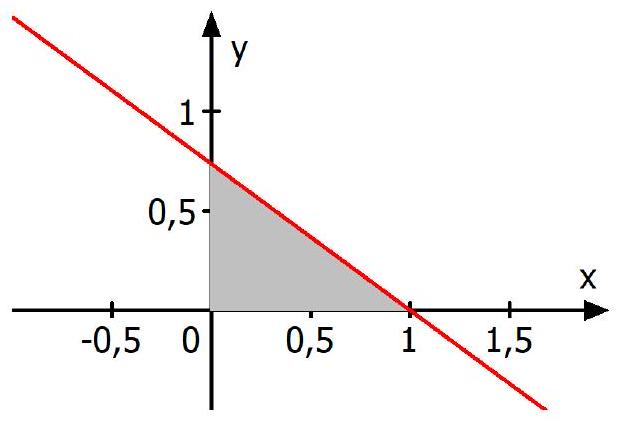
\includegraphics[max width=\textwidth, center]{2025_04_24_90a5eda6f4e325482b12g-5}

Interpretieren Sie in diesem Zusammenhang die Ungleichung geometrisch.\\
Bei der Rotation um die $x$-Achse entsteht ein Kegel mit $h=1$ und $r=\frac{2}{e}$ :\\
$\mathrm{V}_{\mathrm{x}}=\frac{1}{3} \pi \cdot\left(\frac{2}{\mathrm{e}}\right)^{2} \cdot 1=\frac{4 \pi}{3 \mathrm{e}^{2}}$\\
Bei der Rotation um die $y$-Achse entsteht ein Kegel mit $r=1$ und $h=\frac{2}{e}$ :\\
$\mathrm{V}_{\mathrm{y}}=\frac{1}{3} \pi \cdot 1^{2} \cdot \frac{2}{\mathrm{e}}=\frac{2 \pi}{3 \mathrm{e}}$\\
Interpretation der Ungleichung: Das Volumen des Kegels, der bei Rotation der Dreiecksfläche um die y-Achse entsteht ist größer als der Kegel, der bei Rotation um die x-Achse entsteht.\\
d) Berechnen Sie diesen Wert von $t$.

Berechnung der Schnittstellen mit der $x$-Achse: $\mathrm{f}_{\mathrm{t}}(\mathrm{x})=0 \Leftrightarrow\left(1-\mathrm{tx}^{2}\right) \cdot \mathrm{e}^{-2 \mathrm{x}}=0$ Lösung mit dem Satz vom Nullprodukt\\
Gleichung I): $\mathrm{e}^{-2 x}=0$ ist nicht lösbar\\
Gleichung II): $1-\mathrm{tx}^{2}=0 \Leftrightarrow \mathrm{x}_{1,2}= \pm \sqrt{\frac{1}{\mathrm{t}}}$

Der Abstand der Schnittpunkte ist $2 \cdot \sqrt{\frac{1}{t}}$.\\
Bedingung: $2 \cdot \sqrt{\frac{1}{t}}=8 \Leftrightarrow \sqrt{\frac{1}{t}}=4$ |quadrieren

$$
\Rightarrow \frac{1}{t}=16 \Leftrightarrow t=\frac{1}{16}
$$

e) Bestimmen Sie den Inhalt dieser Fläche.

$$
\begin{aligned}
A(z) & =\left|\int_{0}^{2}\left(f_{t}(x)-f_{t+2}(x)\right) d x\right|=\left|\left[-\left(x^{2}+x+\frac{1}{2}\right) \cdot e^{-2 x}\right]_{0}^{z}\right|=\left|-\left(z^{2}+z+\frac{1}{2}\right) \cdot e^{-2 z}-\left(-\frac{1}{2}\right)\right| \\
& =\left|-\left(z^{2}+z+\frac{1}{2}\right) \cdot e^{-2 z}+\frac{1}{2}\right|
\end{aligned}
$$

Für $z \rightarrow+\infty$ gilt $A(z) \rightarrow \frac{1}{2}$\\
f) Begründen Sie, dass der Mittelpunkt der Strecke $P_{t} Q_{t}$ auf der Gerade mit der Gleichung $\mathrm{x}=\frac{1}{2}$ liegt.

Notwendige Bedingung für Extremstellen: $\mathrm{f}_{\mathrm{t}}^{\prime}(\mathrm{x})=0$\\
Es gilt $f_{t}^{\prime}(x)=-2 t x \cdot e^{-2 x}+\left(1-t x^{2}\right) \cdot e^{-2 x} \cdot(-2)=2 e^{-2 x}\left(-t x-1+t x^{2}\right)$.\\
$2 \mathrm{e}^{-2 x}\left(-\mathrm{tx}-1+\mathrm{tx}^{2}\right)=0$ Lösung mit dem Satz vom Nullprodukt\\
Gleichung I): $2 e^{-2 x}=0$ ist nicht lösbar\\
Gleichung II): $\mathrm{tx}^{2}-\mathrm{tx}-1=0 \Rightarrow \mathrm{x}_{1,2}=\frac{\mathrm{t} \pm \sqrt{\mathrm{t}^{2}+4 \mathrm{t}}}{2 \mathrm{t}}$\\
Da in der Aufgabe steht, dass der Graph $G_{t}$ zwei Extrempunkte besitzt, muss die hinreichende Bedingung nicht geprüft werden.

Mittelwert der Extremstellen:

$$
\frac{x_{1}+x_{2}}{2}=\frac{\frac{t+\sqrt{t^{2}+4 t}}{2 t}+\frac{t-\sqrt{t^{2}+4 t}}{2 t}}{2}=\frac{\frac{t+\sqrt{t^{2}+4 t}+t-\sqrt{t^{2}+4 t}}{2 t}}{2}=\frac{\frac{2 t}{2 t}}{2}=\frac{1}{2}
$$

Da der Mittelwert der Extremstellen $\frac{1}{2}$ beträgt, ist der Nachweis erbracht.

\section*{Aufgabe A 1.2}
a) Zeigen Sie, dass alle diese Wendetangenten parallel zueinander sind.

Hinreichende Bedingung für Wendestelle: $f_{k}^{\prime \prime}(x)=0$ und $f_{k}^{\prime \prime \prime}(x) \neq 0$

$$
\begin{aligned}
& f_{k}^{\prime}(x)=-\frac{1}{k^{2}}(x-k)(x+3 k)=-\frac{1}{k^{2}}\left(x^{2}+2 k x-3 k^{2}\right) \\
& f_{k}^{\prime \prime}(x)=-\frac{1}{k^{2}}(2 x+2 k) \\
& f_{k}^{\prime \prime \prime}(x)=-\frac{1}{k^{2}} \cdot 2 \\
& -\frac{1}{k^{2}}(2 x+2 k)=0 \Leftrightarrow 2 x+2 k=0 \Leftrightarrow x=-k
\end{aligned}
$$

$\mathrm{f}_{\mathrm{k}}^{\prime \prime \prime}(-\mathrm{k})=-\frac{2}{\mathrm{k}^{2}} \neq 0$ also existiert bei $\mathrm{x}=-\mathrm{k}$ eine Wendestelle.\\
Steigung der Wendetangente: $f_{k}^{\prime}(-k)=-\frac{1}{k^{2}} \cdot\left(k^{2}-2 k^{2}-3 k^{2}\right)=-\frac{1}{k^{2}} \cdot\left(-4 k^{2}\right)=4$\\
Da die Steigung unabhängig von k ist, sind alle Wendetangenten parallel zueinander.

Hinweis:
Es gibt noch eine weitere Möglichkeit, die Wendestelle $x=-k$ zu erhalten. Die Ableitungsfunktion ist eine ganzrationale Funktion 2.Grades.\\
Somit ist die Funktion f eine ganzrationale Funktion 3.Grades.\\
Solch eine Funktion ist immer zu ihrem Wendepunkt symmetrisch.\\
Mit dem Ansatz $f_{k}^{\prime}(x)=0$ können die Extremstellen des Graphen von $f_{k}$ berechnet werden.

$$
-\frac{1}{k^{2}}(x-k)(x+3 k)=0
$$

Lösung mit dem Satz vom Nullprodukt: $\mathrm{x}_{1}=\mathrm{k}$ und $\mathrm{x}_{2}=-3 \mathrm{k}$\\
Mittelwert der Extremstellen: $\frac{\mathrm{x}_{1}+\mathrm{x}_{2}}{2}=\frac{\mathrm{k}+(-3 \mathrm{k})}{2}=\frac{-2 \mathrm{k}}{2}=-\mathrm{k}$\\
Dies ist die Wendestelle des Graphen von $f_{k}$.\\
b) Bestimmen Sie eine Funktionsgleichung von $f_{k}$.

In a) wurde berechnet: $\mathrm{f}_{\mathrm{k}}^{\prime}(\mathrm{x})=-\frac{1}{\mathrm{k}^{2}}\left(\mathrm{x}^{2}+2 \mathrm{kx}-3 \mathrm{k}^{2}\right)$\\
Alle Stammfunktionen von $f_{k}^{\prime}$ lauten $f_{k}(x)=-\frac{1}{k^{2}} \cdot\left(\frac{1}{3} x^{3}+k x^{2}-3 k^{2} x\right)+C$

Notwendige Bedingung für Extremstellen: $\mathrm{f}_{\mathrm{k}}^{\prime}(\mathrm{x})=0$\\
$-\frac{1}{k^{2}}(x-k)(x+3 k)=0$\\
Lösung mit dem Satz vom Nullprodukt: $\mathrm{x}_{1}=\mathrm{k}$ und $\mathrm{x}_{2}=-3 \mathrm{k}$\\
Da in der Aufgabe vorgegeben ist, dass jeder Graph im 1.Quadrant einen Extrempunkt besitzt, muss der $x$-Wert des Extrempunktes $\mathrm{x}=\mathrm{k}$ sein (wegen k > 0).

Da der Extrempunkt auf der ersten Winkelhalbierenden $y=x$ liegt, lautet der vorgegebene Extrempunkt $\mathrm{E}(\mathrm{k} \mid \mathrm{k})$.

Bedingung: $f_{k}(x)=k$\\
$k=-\frac{1}{k^{2}} \cdot\left(\frac{1}{3} k^{3}+k^{3}-3 k^{3}\right)+C \Leftrightarrow k=\frac{5}{3} k+C \Leftrightarrow C=-\frac{2}{3} k$\\
Gesuchte Funktionsgleichung: $f_{k}(x)=-\frac{1}{k^{2}} \cdot\left(\frac{1}{3} x^{3}+k x^{2}-3 k^{2} x\right)-\frac{2}{3} k$


\end{document}